\documentclass[11pt,a4paper]{article}
\usepackage[margin=2.3cm]{geometry}
\usepackage{amsmath,amssymb}
\usepackage{graphicx}
\usepackage{booktabs}
\usepackage{array}
\usepackage{adjustbox}
\usepackage[hidelinks]{hyperref}
\emergencystretch=3em

\newcommand{\bu}{\boldsymbol{u}}
\newcommand{\bv}{\boldsymbol{v}}
\newcommand{\bb}{\boldsymbol{b}}
\newcommand{\bff}{\boldsymbol{f}}
\newcommand{\bU}{\boldsymbol{U}}
\newcommand{\bud}{\dot{\boldsymbol{U}}}
\newcommand{\dt}{\Delta t}
\newcommand{\code}[1]{\texttt{#1}}
\newcommand{\spg}{\mathrm{spg}}
\newcommand{\be}{\boldsymbol{e}}
\newcommand{\bd}{\boldsymbol{d}}

\title{A posteriori error estimation for SUPG--Taylor--Hood discretisations\\of the time-dependent Navier--Stokes equations:\\
the AAJ27 examples in time, and an implementation of the adaptive\\SUPG/PSPG/grad-div method of the draft (v6)}
\author{galerkit, branch \code{time-navier-stokes}}
\date{November 2026}

\begin{document}
\maketitle

\begin{abstract}
This report continues \code{navier\_stokes/theta\_supg\_th} and documents two further pieces of work on the galerkit
branch \code{time-navier-stokes}. Part~I extends Examples 5.1 and 5.2 of Afzal, Ahmed and John~\cite{AAJ27} to the
time-dependent case and studies, with the SUPG--Taylor--Hood method of the previous report (no PSPG, no grad-div)
and its FGJN14-type estimator (not the AAJ27 estimator), the convergence in space, the effectivity index and the
contributions of the estimator. Part~II is a new implementation (package
\code{galerkit.\allowbreak navier\_stokes.\allowbreak twod.\allowbreak adaptive\_spg\_th}) of the adaptive
SUPG/PSPG/grad-div method of the working draft ``An adaptive SUPG/PSPG/grad-div method for the time-dependent
incompressible Navier--Stokes equations'' (v6, November 2026)~\cite{draft}, for the pair $P_2/P_1$, together with a
review of the draft, an audit of the earlier implementation, and Examples~1--3 of the draft.
All rates and comparisons are \emph{observed numerically}; nothing in this report is a proof. Claims are marked as
\emph{checked} (verified numerically or by a test), \emph{plausible} (consistent with the data, not verified) or
\emph{open}.
\end{abstract}

\tableofcontents

%=====================================================================================================
\part{AAJ27 Examples 5.1 and 5.2 in the time-dependent case}

\section{Setting}
The steady solutions of~\cite[Sect.~5]{AAJ27} are multiplied by $g(t)=1+\frac12\sin 2\pi t$, $\bu(\boldsymbol x,t)=g(t)\boldsymbol U(\boldsymbol x)$,
$p=g(t)P(\boldsymbol x)$, and $\bff$ is computed from the time-dependent Navier--Stokes equations:
Example~5.1 is the smooth solution (35)--(36) of~\cite{AAJ27} ($\nu=10^{-2}$ and $1/400$), Example~5.2 the solution with
boundary layers at $x=1$, $y=1$, $\bu=\operatorname{curl}\phi$, $\phi=x^2y^2(1-e^{\lambda(x-1)})^2(1-e^{\lambda(y-1)})^2$,
$\lambda=0.5/\sqrt\nu$, $p=e^{x+y}-(e-1)^2$. The coarsest mesh is that of AAJ27 (the unit square with one diagonal),
levels 2--7 by red refinement ($188$ to $148\,740$ dofs), $\dt=0.01$, $T=1$, trapezoidal rule.
The discretisation is the SUPG--Taylor--Hood method of the previous report (SUPG with the pressure gradient in the
residual, $\delta_K=0.25\min\{h_K/\|\bu_h\|_{\infty,K},h_K^2/\nu\}$, no PSPG, no grad-div).
The estimator is the extension \code{supg} of FGJN14~(28) (cell residual, edge jumps, divergence term); the AAJ27
estimator (34) is \emph{not} used, as requested.

Three error norms are reported:
the AAJ27 norm $\|\cdot\|_{\spg,\mathrm{nse}}$ of~\cite[Sect.~5]{AAJ27} with $\delta_K=0.5h_K^2$, $\mu_K=0.5$ (a yardstick:
our method has no PSPG/grad-div), the SUPG norm $(\nu|e_u|_1^2+\sum_K\delta_K\|(\bu_h\cdot\nabla)e_u\|_K^2)^{1/2}$, and the
\emph{residual SUPG norm}
\[
\|(e_u,e_p)\|_{\mathrm{res}}=\Bigl(\nu|e_u|_1^2+\sum_K\delta_K\|(\bu_h\cdot\nabla)e_u+\nabla e_p\|_K^2\Bigr)^{1/2},
\]
which contains the pressure where the SUPG residual, and hence the estimator, contains it.

\section{Results}
\begin{table}[htbp]\centering\small
\begin{tabular}{llcccc}\toprule
example & quantity & level 2 & level 5 & level 7 & finest rate\\\midrule
5.1, $\nu=10^{-2}$ & res.\ SUPG norm & 2.84 & 0.432 & 2.85e-2 & 1.99\\
 & $\eta_{\mathrm{supg}}$ & 18.4 & 2.27 & 0.152 & 1.99\\
 & eff (res.) & 6.50 & 5.26 & 5.33 & \\
 & eff (SUPG norm) & 10.6 & 38.1 & 73.5 & \\
 & eff ($\spg,\mathrm{nse}$) & 3.27 & 5.80 & 10.8 & \\\midrule
5.1, $\nu=1/400$ & eff (res.) & 6.58 & 5.63 & 5.37 & \\
 & eff (SUPG norm) & 9.38 & 24.3 & 39.5 & \\\midrule
5.2, $\nu=10^{-2}$ & res.\ SUPG norm & 0.467 & 1.82e-2 & 1.27e-3 & 1.99\\
 & eff (res.) & 7.13 & 7.02 & 6.84 & \\
 & eff (SUPG norm) & 16.1 & 21.8 & 36.6 & \\\bottomrule
\end{tabular}
\caption{Part I, $t=1$, uniform meshes. The effectivity w.r.t.\ the residual SUPG norm varies by at most $\pm0.3$
between $t=0.25,0.5,0.75,1$ on every level.}\label{tab:aaj}
\end{table}

\begin{figure}[htbp]\centering
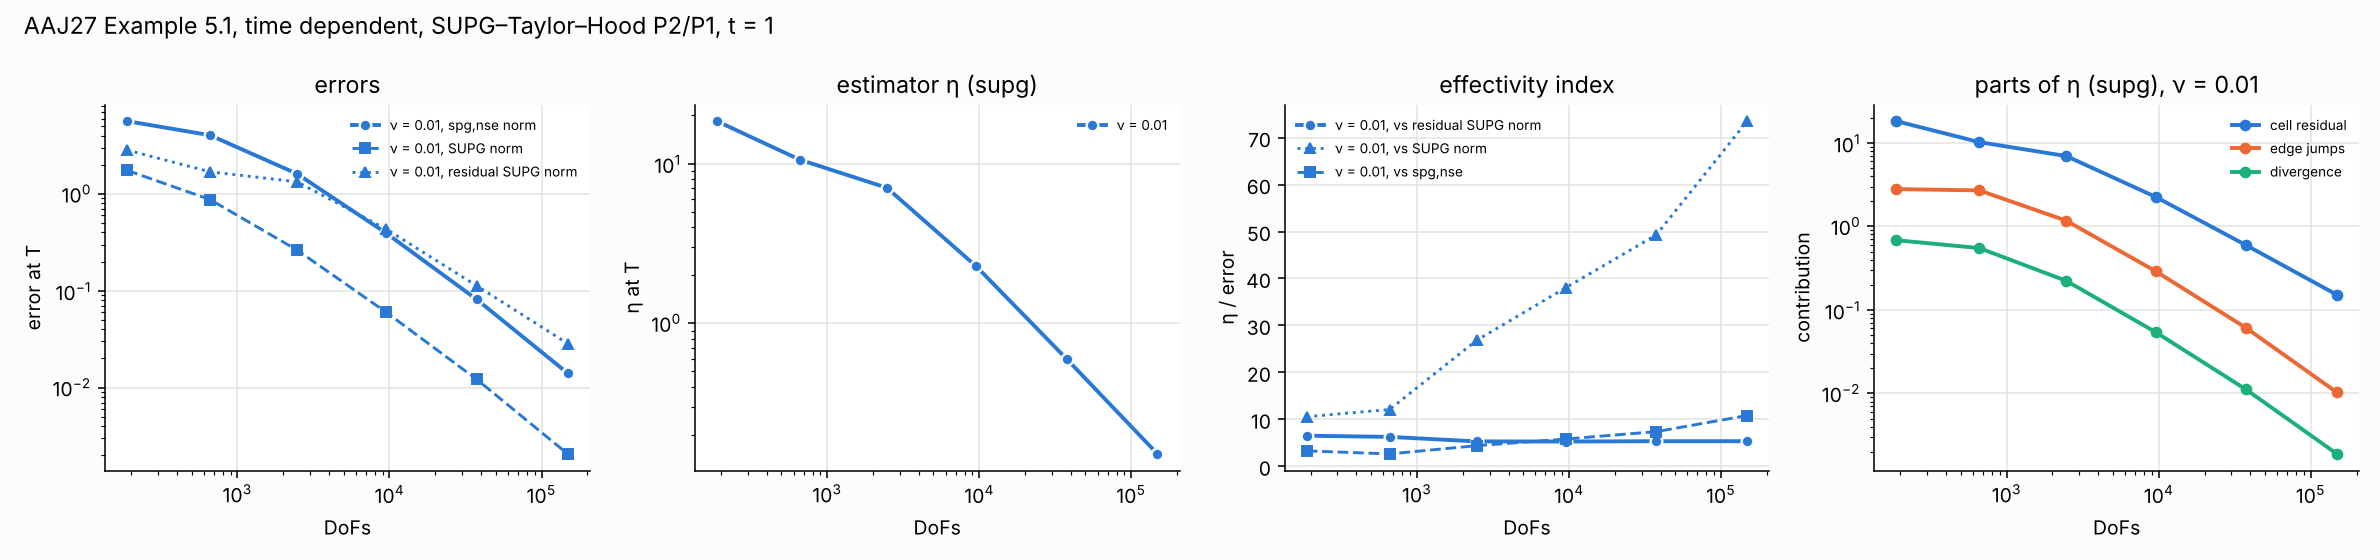
\includegraphics[width=\textwidth]{figures/aaj_ex51_nu1e-2.png}
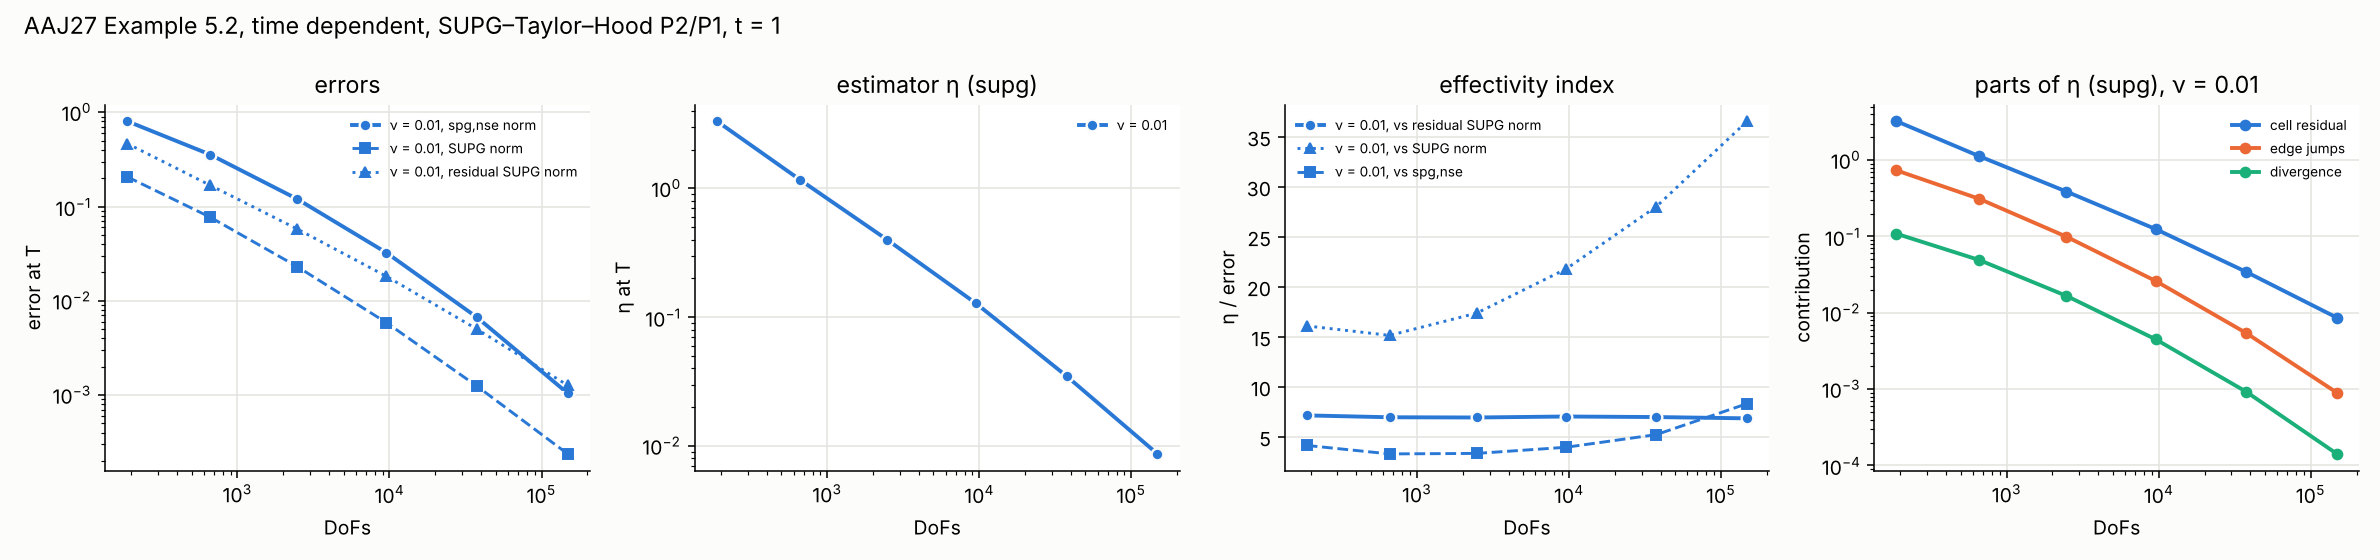
\includegraphics[width=\textwidth]{figures/aaj_ex52_space.png}
\caption{Part I: errors, estimator, effectivity index and contributions; Example 5.1 ($\nu=10^{-2}$, top) and 5.2 (bottom).}
\end{figure}

\paragraph{Observations.}
\begin{enumerate}
\item The effectivity of $\eta_{\mathrm{supg}}$ w.r.t.\ the residual SUPG norm is $5.3$--$7.1$ on all levels, both
viscosities, both examples, all output times and on the adaptive meshes ($5.4$--$6.5$) (\emph{checked}).
\item W.r.t.\ the velocity-only SUPG norm it grows ($10\to74$): the residual contains $\nabla(p-p_h)=O(h)$ for $P_1$
pressure, while the SUPG norm of the velocity error is $O(h^2)$. Replacing $\nabla p_h$ by $\nabla p$ in the residual gave
effectivities $6.4$--$9.3$ (\emph{checked}).
\item The $h^1$ estimator is not robust (effectivity w.r.t.\ the residual norm drifts from $\approx3$ to $0.7$).
\item The cell residual dominates ($\geq90\%$); edge jumps $\approx7\%$, divergence $\approx1\%$.
\item Adaptivity (Example 5.2, D\"orfler marking with $h^1$ ranking and \code{supg} global estimate): at $\approx9.7$k dofs the
energy-type errors are $1.5$--$1.7$ times smaller than on uniform level 5, the $L^2$ velocity error is larger
($7.0\cdot10^{-4}$ vs $3.8\cdot10^{-4}$) (Fig.~\ref{fig:aajad}).
\end{enumerate}

\begin{figure}[htbp]\centering
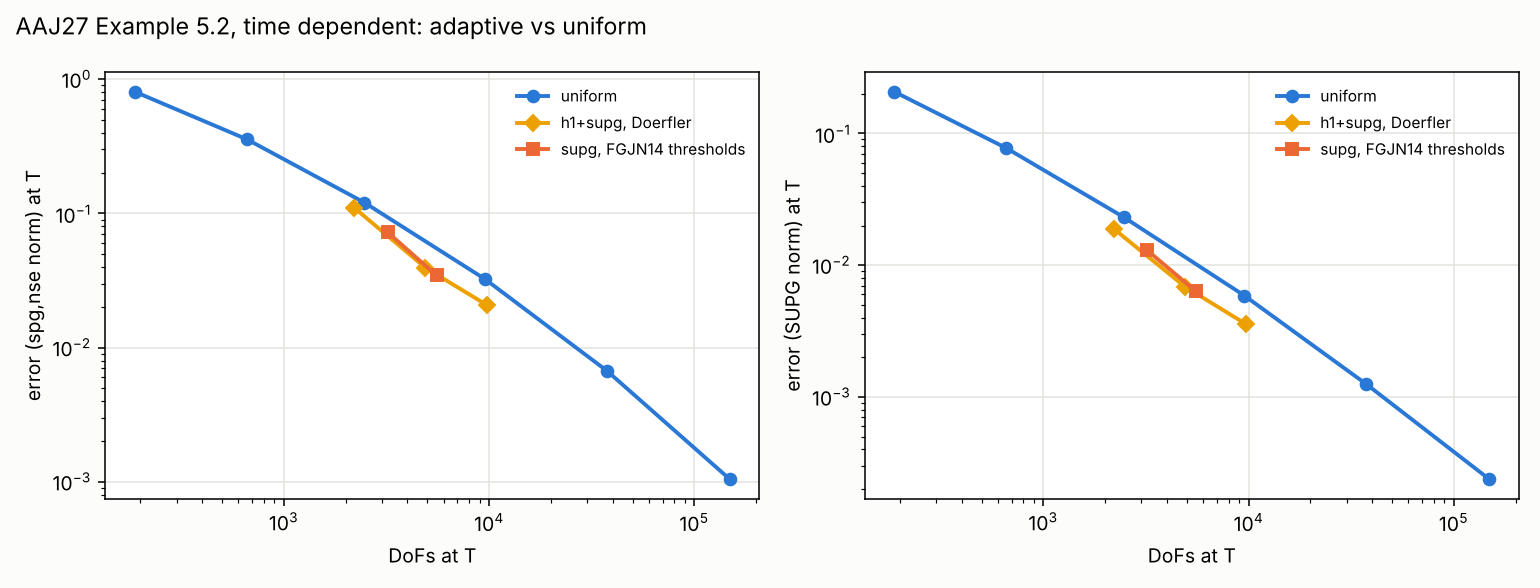
\includegraphics[width=0.62\textwidth]{figures/aaj_ex52_adaptive_vs_uniform.png}
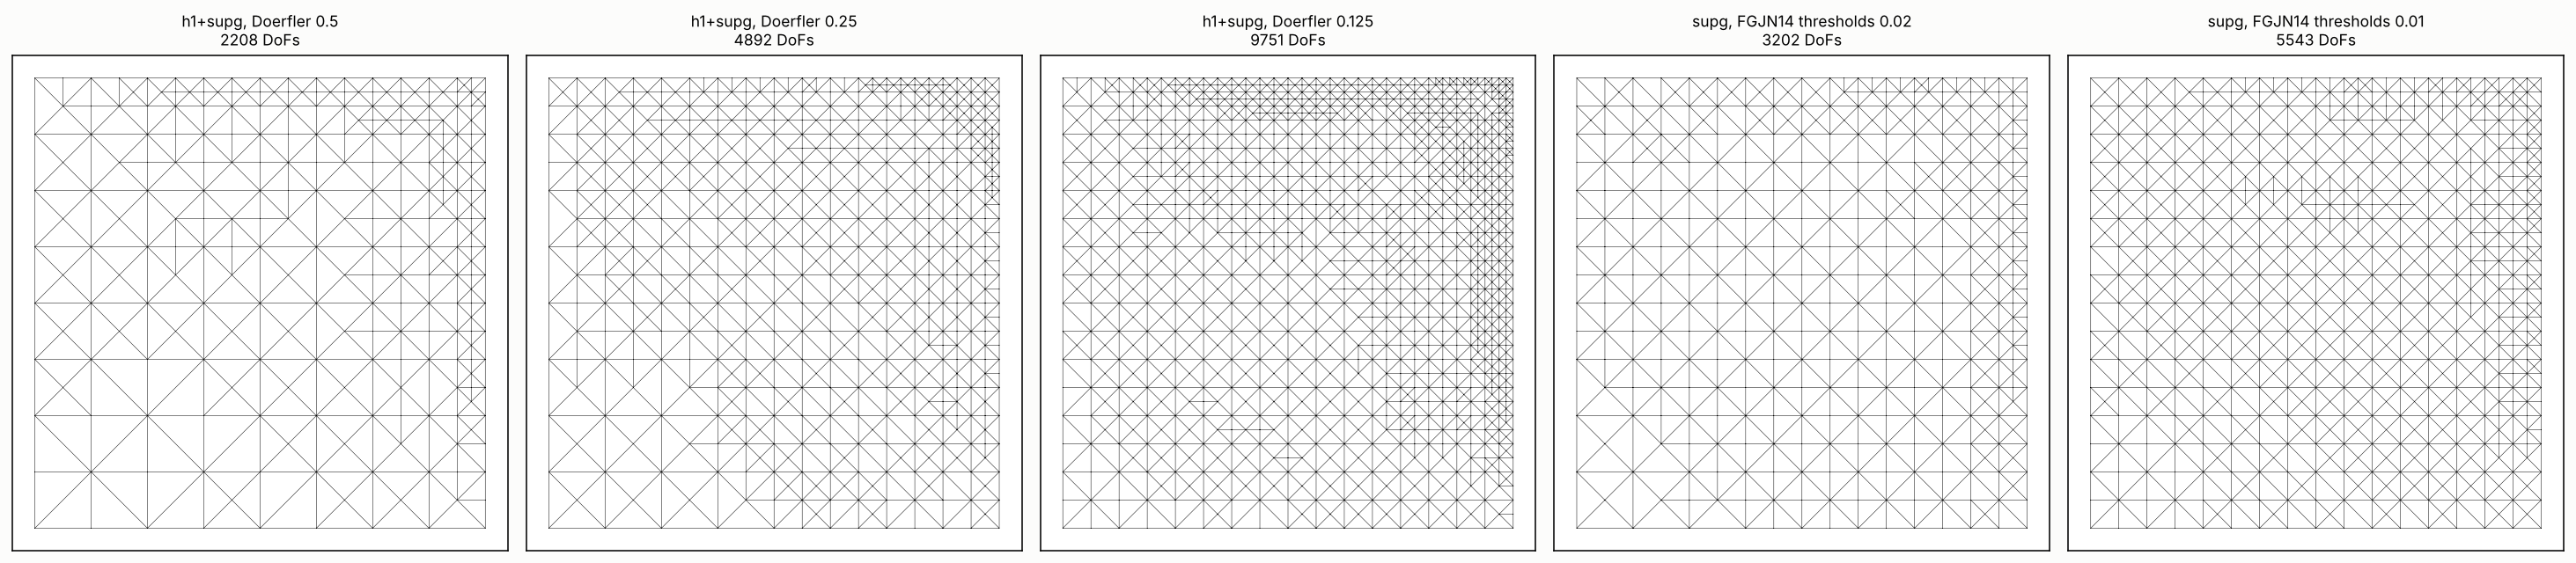
\includegraphics[width=\textwidth]{figures/aaj_ex52_meshes.png}
\caption{Part I, Example 5.2, $\nu=10^{-2}$: adaptive vs uniform, and the adaptive meshes at $t=1$.}\label{fig:aajad}
\end{figure}

\section{Example 5.2 at \texorpdfstring{$\nu=10^{-4}$ and $10^{-6}$}{nu = 1e-4 and 1e-6}}
The exact solution reaches $\max|\bu|\approx19$ ($\nu=10^{-4}$) and $\approx240$ ($\nu=10^{-6}$); the layer width is
$1/\lambda=0.02$ and $0.002$. The degree-7 quadrature under-integrates the layers at $\nu=10^{-6}$ (exact $|\bu|_1$
by $64\%$ on level 2 to $1.5\%$ on level 7), so errors and estimators were evaluated with a composite rule as fine as
level 8 (error $<0.1\%$, \emph{checked}). Newton failures were handled by halving $\dt$ (at most twice). The runs were
stopped after levels 5 ($\nu=10^{-4}$) and 4 ($\nu=10^{-6}$) because the results were not satisfactory:
\begin{center}\small
\begin{tabular}{lcccccc}\toprule
$\nu$ & level & dofs & $\spg,\mathrm{nse}$ & SUPG norm & $\eta_{\mathrm{supg}}$ & eff (res.)\\\midrule
$10^{-4}$ & 2 & 188 & 20.8 & 12.8 & 201 & 14.5\\
 & 5 & 9540 & 55.2 & 27.7 & 57.1 & 3.05\\
$10^{-6}$ & 2 & 188 & 29.4 & 20.3 & 24\,910 & 1285\\
 & 4 & 2468 & 453 & 204 & 5\,317 & 25.8\\\bottomrule
\end{tabular}
\end{center}
All errors grow under refinement on these levels (the layers are not resolved), $\eta$ decreases, and the effectivity
is not robust in this pre-asymptotic regime. Plausible (not checked): the cell residual is dominated by the data
$\bff$ ($\approx10^7$ near the layers at $\nu=10^{-6}$). AAJ27 report Navier--Stokes results only for $\nu\ge1/400$.

%=====================================================================================================
\part{The adaptive SUPG/PSPG/grad-div method of the draft (v6)}

\section{Review of the draft}
The derivations of Lemma~lem:prelim and Theorem~thm:upper were re-derived step by step: the Young constants
($ab\le2a^2+b^2/8$, $xy\le10x^2+y^2/40$), the absorption of (H0), the weights $320$, $160$, $640$, the bound
$|\Psi(\be)|\le\kappa E^2$ and the factor $(1-8\kappa)^{-1}$. No error was found (\emph{checked} by hand).
Points that matter for an implementation:
\begin{enumerate}
\item Example~2 asks for the marking of~\cite[Sect.~4.2]{AAJ27} (relax until $\ge10\%$ of the cells are marked) at every
time step; this has no coarsening and no stopping rule and contradicts the threshold marking of Section~4. The
threshold marking of Section~4 was used.
\item $\eta_{\mathrm{div}}=640h^{-2}\max_K\delta_K\|\nabla\cdot\bU\|^2$ with $h=\min_Kh_K$: on graded meshes the factor
$h^{-2}\max\delta_K$ grows like $(h_{\max}/h_{\min})^2$ and couples all cells (observed in Sect.~\ref{sec:ex2}).
\item The initial data: Section~2.4 computes $(\bud^0,P^0)$ from (eq:semi) at $t=0$. Only $\bud^0$ is used by the scheme
($P^0$ is only the first Newton iterate; results with $P^0=0$ differ by $10^{-12}$, \emph{checked}). With PSPG,
$\|\nabla\cdot\bU^0\|=O(h^2)$ and $\delta_K=O(h^2)$ force an $O(1)$ strong residual, so $\bud^0$ has an $O(1)$ error that does
not decrease with $h$ (\emph{checked}: $\|\bud^0-\partial_t\bu(0)\|\approx10$ vs $\|\partial_t\bu\|=2.35$ on levels 2--6),
with consequences in Sect.~\ref{sec:start}.
\item Several statements in the draft are prophetic for the numerics: Remark~rem:dtsupg(ii) (BGL07, $\dt\ge\alpha\delta$),
Remark~rem:transfer (undamped $(-1)^n$ mode after mesh changes), and the non-robustness of (H6).
\end{enumerate}

\section{Audit of the earlier implementation (\code{theta\_th})}
\begin{itemize}
\item \textbf{Bug, fixed:} the estimator and the SUPG norm recomputed $\delta_K$ from the final velocity, while the discrete
solution satisfies the auxiliary problem only with the $\delta_K$ of the step (frozen from the predictor). Now the step's
$\delta_K$ is used.
\item \textbf{Bug, fixed:} the indicator was evaluated with the GGS08-averaged state; it now uses the non-averaged TR solution
(also in the final record when the loop is left after an averaged step).
\item \textbf{Not bugs (checked):} the Galerkin pressure coupling $-(\nabla\cdot\bv,p)$, $(\nabla\cdot\bu,q)$, the SUPG pressure
term, the component-wise loads and the SUPG mass terms agree with a direct evaluation of the forms at the quadrature points
(random fields, cell-dependent parameters, mixed cell orientations) to $10^{-14}$ relative.
\end{itemize}
All three items are regression tests now (\code{tests/test\_ns2d\_adaptive\_spg\_th.py}).

\section{Implementation}
\begin{itemize}
\item \textbf{Scheme} (\code{scheme.py}): the forms (eq:Aspg), (eq:Lspg) with PSPG and grad-div, the TR step (eq:TR) with the
discrete derivative (eq:udot) written as $R(x)=(\sigma M_t(\bb)+K_t(\bb))x-F(\bb)-M_t(\bb)[H;0]$, $\sigma=2/\dt$,
$H=\sigma\bU^n+\bud^n$, Picard (the draft) and Newton (exact Jacobian, same fixed point), stopping on
$\|R\|_2\le10^{-10}$ with a round-off floor $10^{-13}\|\mathrm{rhs}\|$ (addition: the absolute test is unreachable for
large right-hand sides). $\delta_K=\min\{0.5h_K^2,h_K^2/(8C_{\mathrm{inv},K}^2\nu)\}$ (eq:deltacond), $\mu_K=0.5$, with the
inverse constant computed exactly per cell (rank-one generalised eigenproblem; $C_{\mathrm{inv}}=\sqrt{96}$ on the AAJ27
cells with $h_K$ = diameter, so (eq:deltacond) binds at $\nu=10^{-2}$: $\delta_K=0.130h_K^2$). These parameters do not depend
on the velocity, so ``evaluating them with the AB2 predictor'' is void.
\item \textbf{Estimator} (\code{estimator.py}): $\eta_K$ of (eq:etaK) with $C=1$, $d=2$, $\alpha=0$, facet weights $\omega_F$,
Neumann facets, the (A1) check; optional cell-local $\eta_{\mathrm{div}}$ (not the draft, diagnostic).
\item \textbf{Time control} (\code{timestep.py}): TR-AB2 as in Section~4 (rejection if $\|\epsilon\|>TOL_T$, factor $0.85$,
averaging, lower bound $\dt\ge\alpha\min\delta_K$, the non-averaged state for the estimator).
\item \textbf{Algorithm} (\code{adaptive.py}): Section~4 with newest-vertex bisection, interpolation of $\bU,\bud^{n+1},\bud^n$;
options (a) recompute $\bud$ from (eq:semi) after a mesh change and (b) one backward Euler step after a mesh change
(Remark rem:transfer); domains: unit square, cylinder channel (polygonal cylinder, new boundary vertices projected).
\item \textbf{Checks} (\code{checks.py}): (H0)--(H5), $\Theta_h$, the bound (eq:upper) and the ratio of (eq:heur), with $\tilde\bu$
from (eq:aux) on the mesh refined twice ($P_2/P_1$; the draft asks for a higher order pair on the same mesh) and nodal
interpolation.
\end{itemize}
\paragraph{Verification (\emph{checked}, 15 unit tests).} Polynomial solution ($\bu\in P_2$, $p\in P_1$, linear in $t$)
reproduced to $10^{-11}$ including $\bud^0,P^0$; Newton Jacobian against finite differences ($<10^{-7}$); Picard $=$ Newton
($10^{-11}$); Lemma~lem:exact: the TR solution satisfies (eq:disc-aux) to $10^{-11}$, and the auxiliary problem solved on the
same mesh returns the TR solution; the estimator vanishes for the exact discrete solution; the backward Euler step satisfies
(eq:semi); forms against direct quadrature evaluation.

\section{Example 1: smooth solution, uniform meshes}
AAJ27 (35)--(36) with $(1+\frac12\sin\pi t)$ (velocity) and $(1+\frac12\cos\pi t)$ (pressure), $T=2$, $\dt=10^{-3}$, levels
2--6, start as in the draft ($\bud^0$ from (eq:semi)).
\begin{table}[htbp]\centering\small
\adjustbox{max width=\textwidth}{\begin{tabular}{lccccc}\toprule
$\nu$ & spg error, level $2\to6$ & rates & $\eta$ rates & eff, levels 2--5 & eff, level 6\\\midrule
$10^{-2}$ & 2.38, 0.769, 0.223, 5.89e-2, 2.79e-2 & 1.80, 1.88, 1.97, \textbf{1.09} & 1.80--2.01 & 19.7--20.0 & \textbf{10.7}\\
$10^{-3}$ & 4.09, 1.29, 0.415, 0.102, 2.69e-2 & 1.84, 1.72, 2.07, 1.95 & 1.81--1.98 & 20.3--22.7 & 21.2\\
$10^{-4}$ & 4.14, 1.31, 0.403, 0.108, 2.67e-2 & 1.84, 1.79, 1.95, 2.04 & 1.80--2.01 & 20.3--22.6 & 20.7\\\bottomrule
\end{tabular}}
\caption{Example 1, $t=2$ (start as in the draft). The contributions are ordered $\eta_{\mathrm{res}}>\eta_\delta>\eta_{\mathrm{div}}>\eta_\mu\gg\eta_F$.}\label{tab:ex1}
\end{table}

\begin{figure}[htbp]\centering
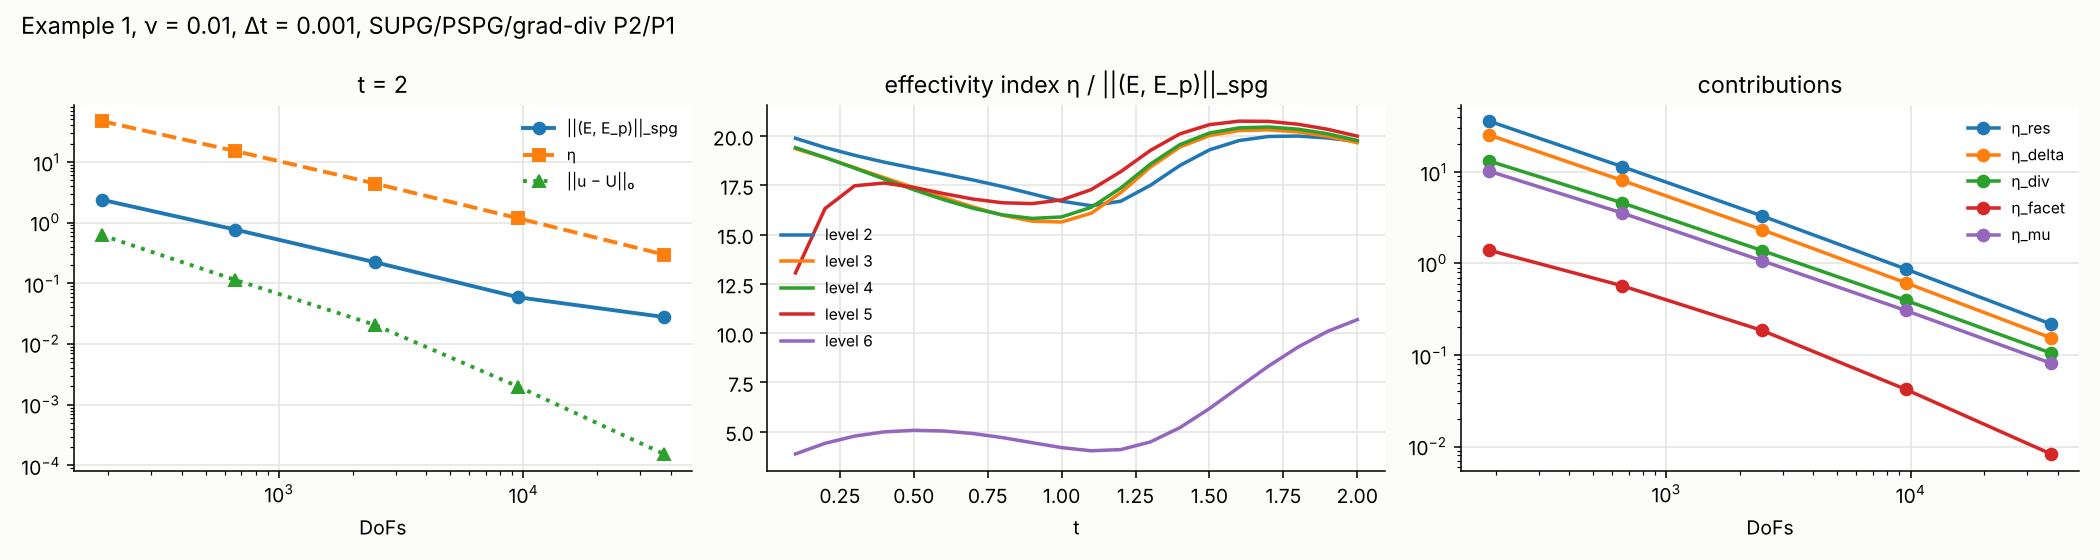
\includegraphics[width=\textwidth]{figures/ex1_nu1e-2.png}
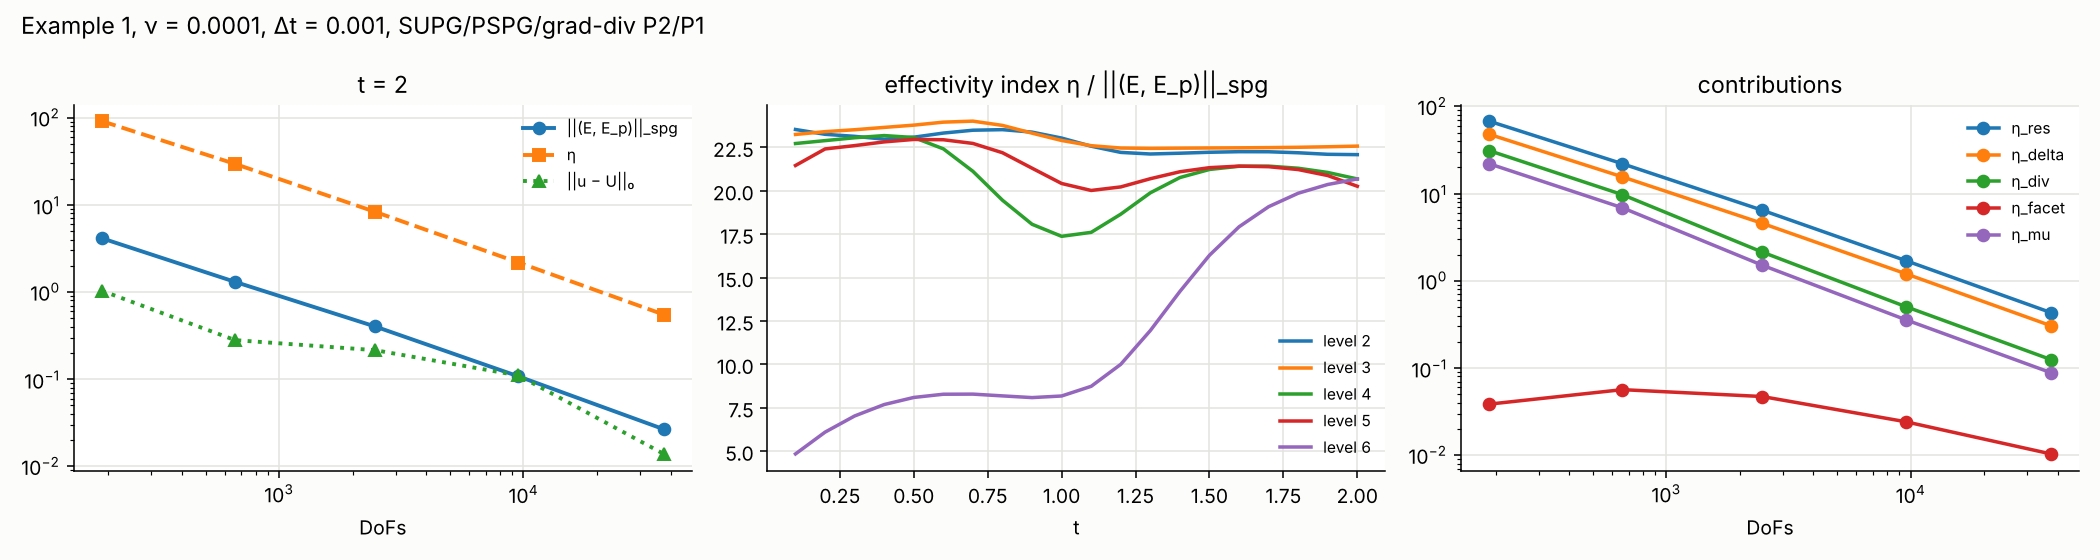
\includegraphics[width=\textwidth]{figures/ex1_nu1e-4.png}
\caption{Example 1, $\nu=10^{-2}$ (top) and $10^{-4}$ (bottom): error and estimator, effectivity versus $t$, contributions.}
\end{figure}

On levels 2--5 the effectivity is $\approx20$ for all $\nu$ and all $t$ ($17$--$24$): about $2.3$ times the $\approx9$ of AAJ27,
consistent with the eight times larger constants of the draft ($\sqrt8\approx2.8$). On level 6 it is $4$--$10$ ($\nu=10^{-2}$)
and rises from $5$ to $21$ ($\nu\le10^{-3}$) over $[0,2]$; Sect.~\ref{sec:start} identifies the cause.

\paragraph{Hypotheses.} $\nu=10^{-2}$, levels 2--5, $t=1,2$: (H0) $\le5\cdot10^{-3}$, (H1) $0.12$--$0.41$, (H3) $\le0.22$, (H4)
$0.2$--$0.75$ hold; (H2) fails ($2.6$--$6.1$, required $\le2$; only at $t=2$ on levels 4--5 it is $1.7$--$1.9$); (H5) holds at $t=1$ ($0.86$--$1.22$) and fails at $t=2$
on levels 3--5 ($3.0$--$3.7$); $\Theta_h\ll\eta$; the bound (eq:upper) holds with a large margin ($\|e\|^2/(\eta^2+\Theta^2)\approx0.003$); the
neglected part $\|(\bd,\pi)\|/\|e\|=0.14$--$0.43$ supports (eq:heur). For $\nu\le10^{-3}$ the steady auxiliary problem is often
not solved from the TR solution (Newton and Picard fail) or a different solution is found (level 3, $\nu=10^{-3}$: auxiliary
error $9.7$, larger than the full error); where solved, (H2) reaches $60$ ($\nu=10^{-4}$) and $\|(\bd,\pi)\|/\|e\|=0.6$--$0.99$,
so (eq:heur) is not supported. This is consistent with the non-robustness of (H6) stated in the draft.

\section{The start of the TR scheme}\label{sec:start}
On level 6 the pressure error starts at $1.1$--$1.4$ and decays slowly ($\nu=10^{-2}$: still $0.54$ at $t=2$), and the spg error is
dominated by its $\delta_K\|(\bU\cdot\nabla)E+\nabla E_p\|$ part. Three starts were compared (level 6, $\nu=10^{-2}$, $\dt=10^{-3}$, $t\le0.3$):
\begin{center}\small
\adjustbox{max width=\textwidth}{\begin{tabular}{lcccc}\toprule
start & $\|p-P\|_0$, $t=0.01/0.3$ & $\|\bud-\partial_t\bu\|_0$, $t=0.3$ & spg error, $t=0.3$ & effectivity\\\midrule
$\bud^0$ from (eq:semi) (draft) & 1.45 / 1.24 & 7.2 & 5.93e-2 & 3.1--5.0\\
one backward Euler step ($\bU^0$ only) & 3.1e-3 / 2.6e-3 & 2.0e-3 & 1.60e-2 & 18.7--20.1\\
$\bud^0$ = interpolant of $\partial_t\bu(0)$ & 3.1e-3 / 2.7e-3 & 4.0e-3 & 1.60e-2 & 18.7--20.1\\\bottomrule
\end{tabular}}
\end{center}
The velocity error is the same in all three ($1.0\cdot10^{-4}$ at $t=0.3$). The level-6 drop of the effectivity is caused
entirely by $\bud^0$ from (eq:semi), whose $O(1)$ error the trapezoidal rule damps only slowly on fine meshes (\emph{checked}).
Plausible mechanism (not proved): the mode is stiff with $z\sim\dt/\delta_K$ ($\approx16$ on level 6, $4$ on level 5 at
$\nu=10^{-2}$), and $|R(z)|\to1$. \textbf{Recommendation for the draft:} start with one backward Euler step, which needs only
$\bu_0$ (or take $\bud^0=\partial_t\bu_0$ if known). A rerun of Example 1 with this start was stopped after levels 2--5, whose
values at $t=2$ coincide with those of Table~\ref{tab:ex1} to all printed digits.

\section{Example 2: boundary layers, adaptive}\label{sec:ex2}
AAJ27 Sect.~4.2 solution times $(1+\frac12\sin\pi t)$ (pressure also), $T=1$, $TOL_T=10^{-5}$, threshold marking
($TOL_2=TOL_1/20$).

\paragraph{The algorithm as written.} $\nu=10^{-2}$ (level0 3, $TOL_1=0.05$) runs: $\approx1000$ cells refined at $x=1$, $y=1$,
effectivity $\approx22$ after $t\approx0.15$ (Fig.~\ref{fig:ex2a}). $\nu=10^{-3}$ blows up: the first step uses
$\dt_0=\min\delta_K=0.0156$ from the inconsistent $\bud^0$; the step control then drives $\dt$ to $10^{-7}$, far below
$\delta_K$ (the BGL07 regime of Remark rem:dtsupg(ii)); all cells exceed $TOL_1$ and the mesh doubles every step;
$\bud$ grows to $10^6$. (An intermediate hypothesis that $\eta_{\mathrm{div}}$ drives this runaway was refuted: the mesh refines
uniformly there and both $\eta_{\mathrm{div}}$ variants coincide.)

\begin{figure}[htbp]\centering
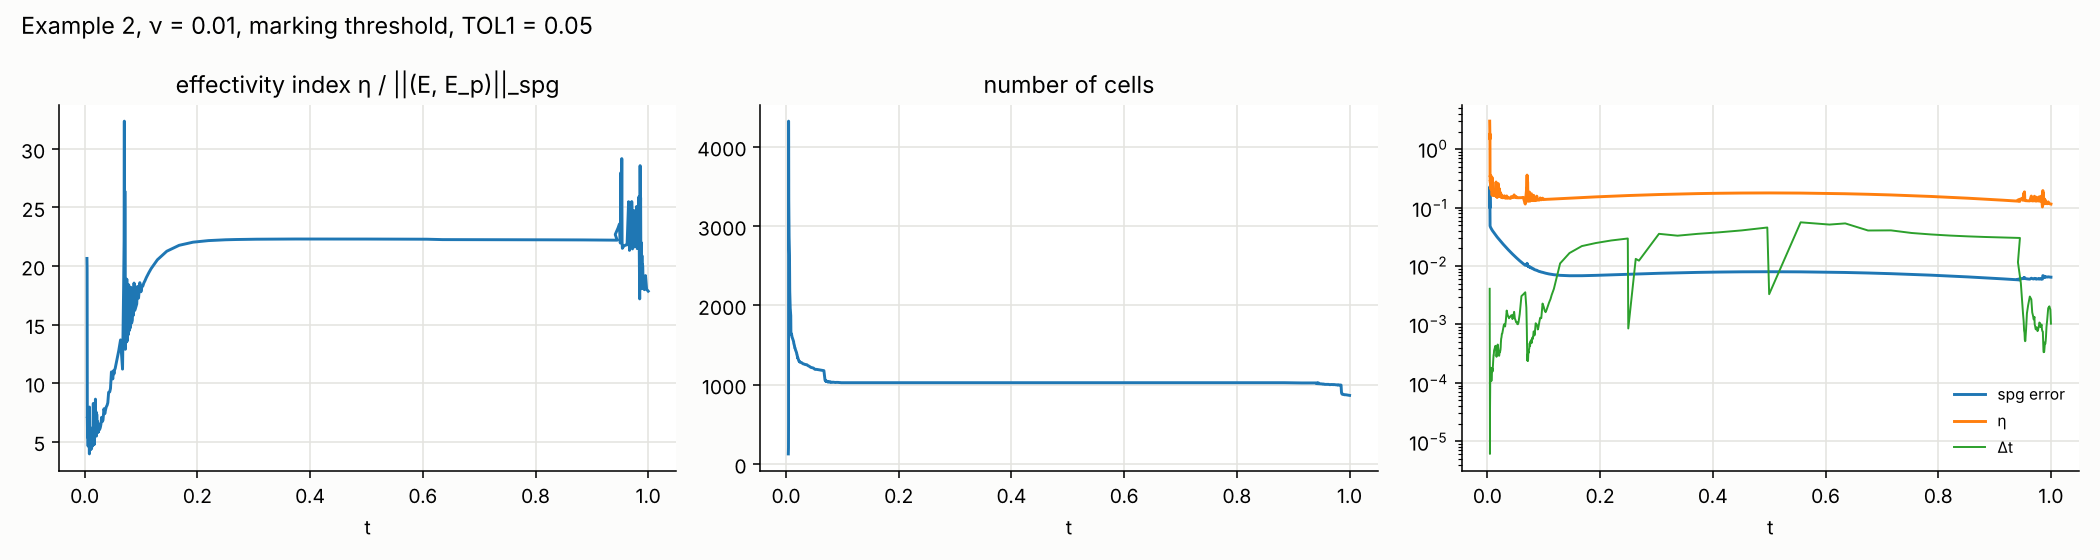
\includegraphics[width=\textwidth]{figures/ex2_nu1e-2_draft_history.png}
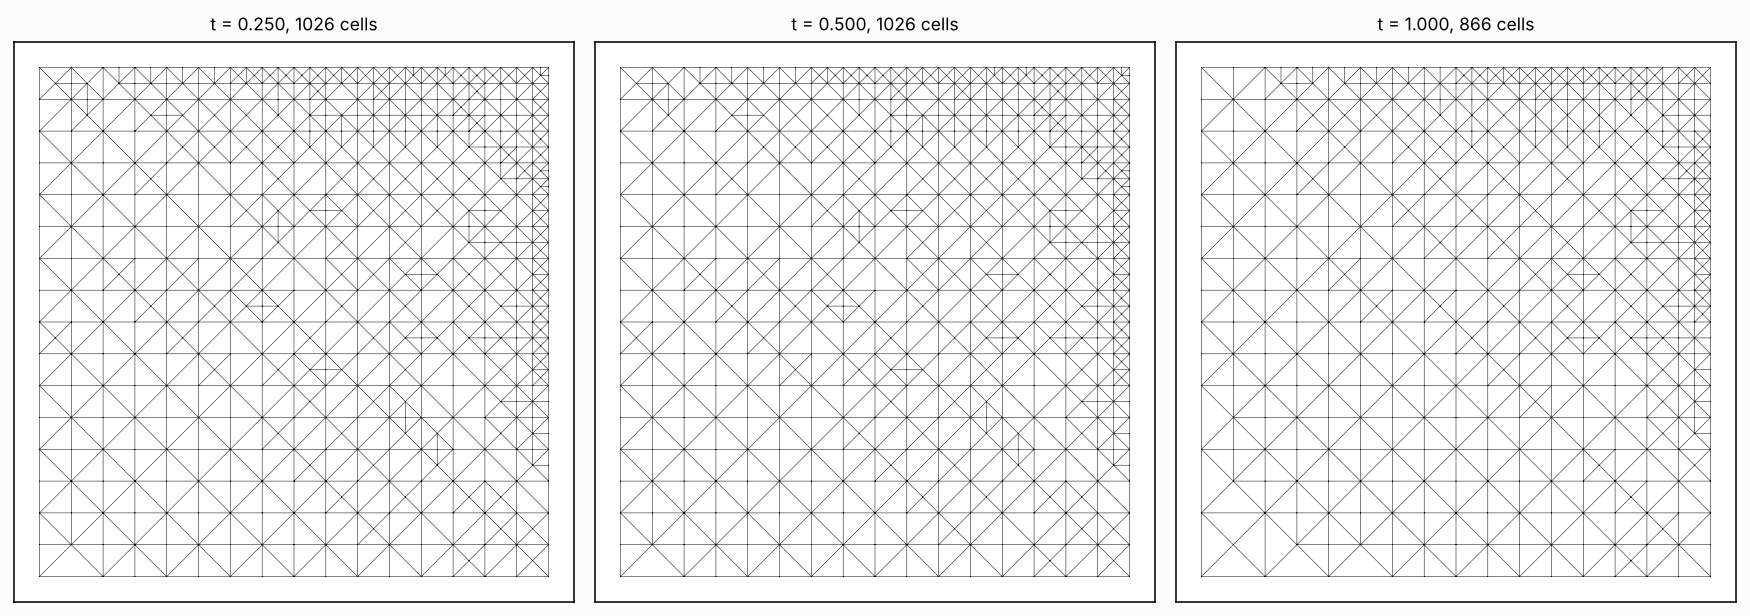
\includegraphics[width=0.85\textwidth]{figures/ex2_nu1e-2_draft_meshes.png}
\caption{Example 2, $\nu=10^{-2}$, algorithm as written: effectivity, cells, errors and step sizes; meshes.}\label{fig:ex2a}
\end{figure}

\paragraph{With (a) + (b).} Recompute $\bud$ from (eq:semi) after every mesh change, one backward Euler step after every
mesh change, $\dt\ge0.1\min\delta_K$, initial mesh level 4 (with level 3 the first step on $h\approx0.18$, wider than the
layer $0.063$, creates an error that is carried along: $\|\bu-\bU\|_0\approx0.3$--$0.45$):
\begin{center}\small
\adjustbox{max width=\textwidth}{\begin{tabular}{lccccc}\toprule
run & steps (damping) & cells & eff, $t>0.1$ & spg error ($T$) & $\|\bu-\bU\|_0$ ($T$)\\\midrule
$\nu=10^{-2}$, $TOL_1=0.05$ & 46 (2) & 524 & 11.1--11.3 & 1.27e-2 & 1.15e-3\\
$\nu=10^{-3}$, $TOL_1=0.3$ & 417 (99) & $\approx990$ & 18.5--29.5 & 9.42e-2 & 0.145\\
$\nu=10^{-3}$, cell-local $\eta_{\mathrm{div}}$ (not the draft) & 315 (35) & $\approx520$ & 7.8--12.2 & 0.154 & 0.202\\\bottomrule
\end{tabular}}
\end{center}
Stable for both viscosities. The draft's $\eta_{\mathrm{div}}$ is $\approx95\%$ of $\eta$ on graded meshes and makes the
effectivity drift with the grading; the cell-local variant gives an effectivity close to the uniform case. The $L^2$
velocity error grows over $[0,1]$ at $\nu=10^{-3}$ in both variants (\emph{open}).

\begin{figure}[htbp]\centering
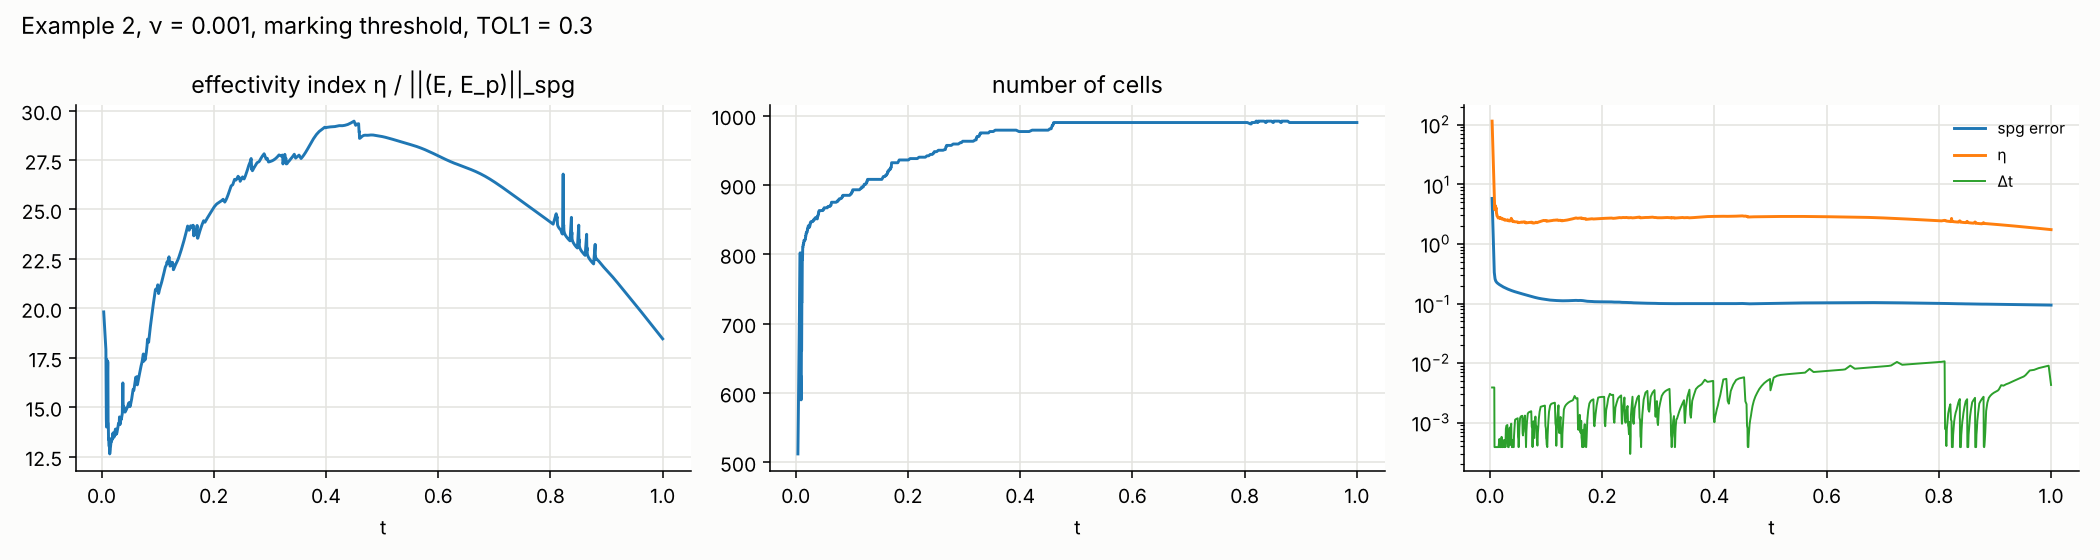
\includegraphics[width=\textwidth]{figures/ex2_nu1e-3_ab_history.png}
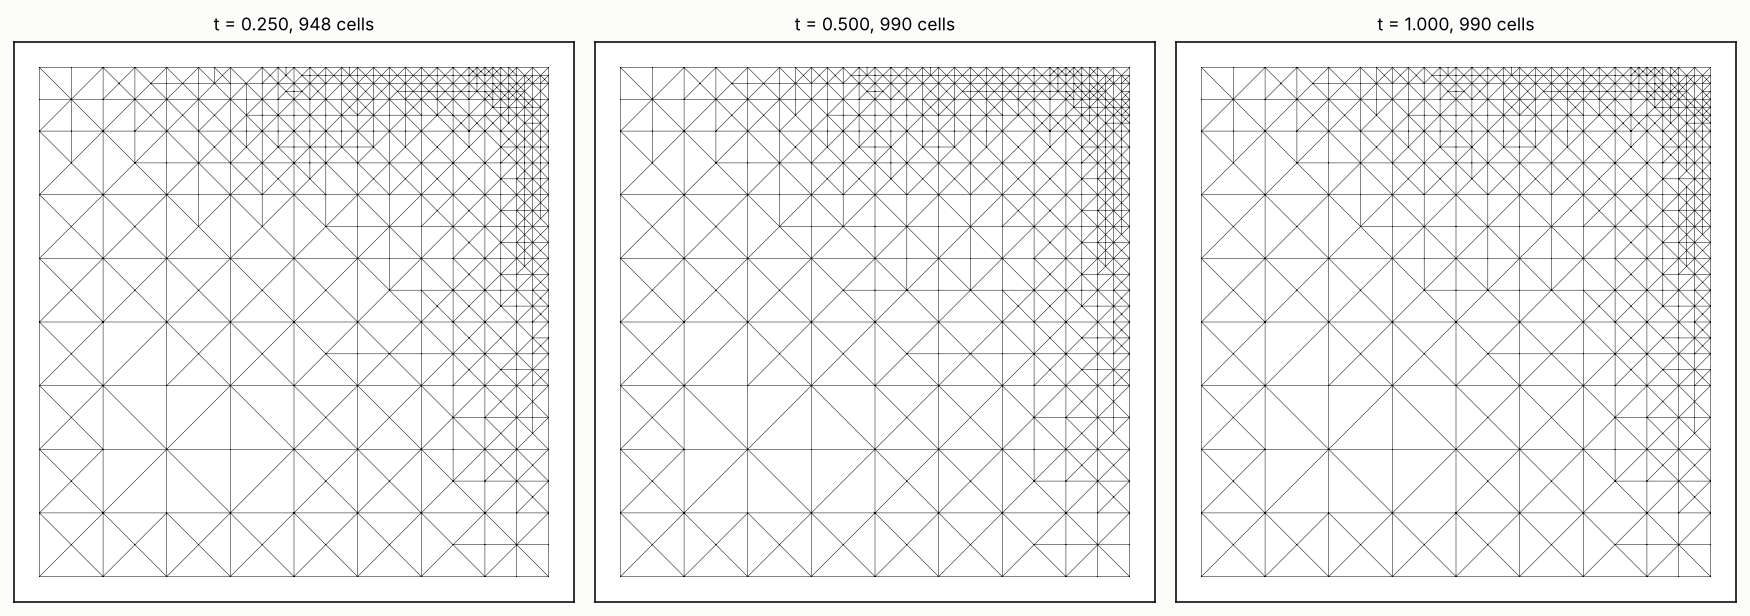
\includegraphics[width=0.85\textwidth]{figures/ex2_nu1e-3_ab_meshes.png}
\caption{Example 2, $\nu=10^{-3}$, with (a)+(b), draft $\eta_{\mathrm{div}}$.}
\end{figure}

\section{Example 3: flow around a cylinder}
ST96 2D with inflow $1.5\sin(\pi t/8)$, $\nu=10^{-3}$, do-nothing outflow, $T=8$, TR-AB2 with $TOL_T=10^{-5}$, $\dt\le0.05$,
(a)+(b), $\dt\ge0.1\min\delta_K$. The cylinder is a polygon with vertices on the circle (affine elements). Drag and lift are
computed from the residual of the stabilised momentum equation tested with a function that is $1$ on the cylinder.
\begin{center}\small
\adjustbox{max width=\textwidth}{\begin{tabular}{lcccccc}\toprule
mesh & dofs & $c_{d,\max}$ ($t$) & $c_{l,\max}$ ($t$) & $\Delta p(8)$ & steps & (A1) violated\\\midrule
uniform level 1 & 5\,082 & 2.8942 (3.918) & 0.4752 (5.842) & $-0.11269$ & 914 & 16.3\%\\
uniform level 2 & 19\,668 & 2.9301 (3.925) & 0.4145 (5.910) & $-0.11352$ & 1052 & 21.6\%\\
reference~\cite{John2016} & & 2.950918 (3.93625) & 0.477875 (5.69250) & $-0.111616$ & & \\\bottomrule
\end{tabular}}
\end{center}
Drag and $\Delta p$ are within $1$--$2\%$. The lift maximum is worse and later on level 2; plausible causes (not checked): $\dt$
up to $0.03$ under-resolves the shedding period $\approx0.3$, damping by grad-div ($\mu=0.5$) and PSPG, the polygonal
cylinder. (A1) is violated in $16$--$22\%$ of the steps, so the upper bound of the draft does not cover them.
The adaptive run (level0 1, $TOL_1=0.1$) failed at $t\approx1.96$: $\dt$ pinned at $0.1\min\delta_K\approx9\cdot10^{-6}$
near the refined cylinder, then the mesh jumped from $3\,900$ to $30\,000$ cells and Newton diverged.

\begin{figure}[htbp]\centering
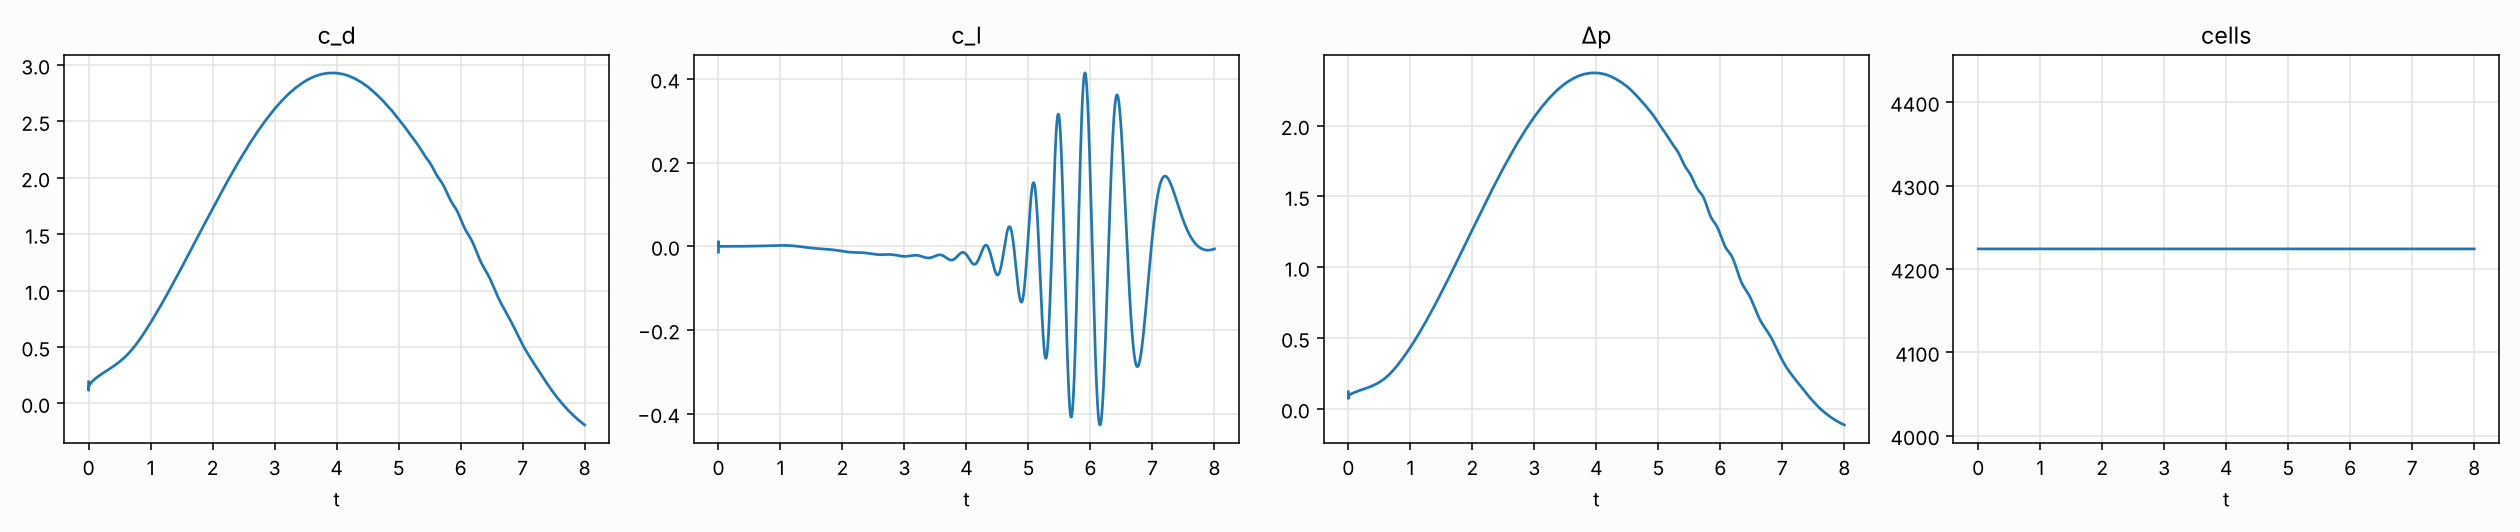
\includegraphics[width=\textwidth]{figures/ex3_l2.png}
\caption{Example 3, uniform level 2: $c_d$, $c_l$, $\Delta p$ versus $t$.}
\end{figure}

\section{Summary}
\begin{itemize}
\item The implementation of the draft (P2/P1) is verified (15 tests). Two bugs of the earlier implementation were fixed; the
pressure coupling and the load assembly were correct.
\item Example 1: the estimator is robust in $h$ and $\nu$ on uniform meshes (effectivity $\approx20$), once the TR scheme is
started with a backward Euler step instead of $\bud^0$ from (eq:semi). (H2) and, at $t=2$, (H5) fail by moderate factors; the
bound holds with a large margin. For $\nu\le10^{-3}$ the auxiliary steady problem is often not solvable and (eq:heur) is not
supported, as anticipated by the non-robustness of (H6).
\item Example 2: the algorithm as written fails at $\nu=10^{-3}$; with (a)+(b), $\dt\ge0.1\min\delta_K$ and a sufficiently
fine initial mesh it is stable. The global weight of $\eta_{\mathrm{div}}$ dominates on graded meshes.
\item Example 3: uniform meshes give drag and $\Delta p$ within $1$--$2\%$; the adaptive run fails.
\item Suggested changes to the draft: backward Euler start; a local weight for $\eta_{\mathrm{div}}$ on graded meshes (would need
a modified proof); a consistent marking for Example 2; dropping PSPG for inf-sup stable pairs (keeping SUPG and grad-div) to
remove the $\dt\ge\alpha\delta$ conflict with the step size control.
\end{itemize}

\paragraph{Reproduction.} galerkit branch \code{time-navier-stokes}:
\begin{itemize}
\item Part I: \code{examples/\allowbreak navier\_stokes/\allowbreak 2d/\allowbreak aaj27\_time/\allowbreak aaj27\_time.py};
\item Part II: \code{examples/\allowbreak navier\_stokes/\allowbreak 2d/\allowbreak adaptive\_spg\_th/\allowbreak example1.py},
\code{example2.py}, \code{example3.py}, with the options \code{-{}-start be}, \code{-{}-recompute-derivative},
\code{-{}-damping}, \code{-{}-dt-min-factor}, \code{-{}-div-local};
\item tests: \code{tests/\allowbreak test\_ns2d\_adaptive\_spg\_th.py}.
\end{itemize}

\begin{thebibliography}{99}
\bibitem{draft} An adaptive SUPG/PSPG/grad-div method for the time-dependent incompressible Navier--Stokes equations,
working draft, version 6, November 2026 (Sections 2--6).
\bibitem{AAJ27} M.~Afzal, N.~Ahmed, V.~John, A robust a posteriori error estimator for the Oseen problem, Comput.\ Math.\ Appl.\ 223 (2026) 467--486.
\bibitem{FGJN14} J.~de Frutos, B.~Garc\'{\i}a-Archilla, V.~John, J.~Novo, An adaptive SUPG method for evolutionary convection--diffusion equations, Comput.\ Methods Appl.\ Mech.\ Engrg.\ 273 (2014) 219--237.
\bibitem{GGS08} P.~M.~Gresho, D.~F.~Griffiths, D.~J.~Silvester, Adaptive time-stepping for incompressible flow. I. Scalar advection--diffusion, SIAM J.\ Sci.\ Comput.\ 30 (2008) 2018--2054.
\bibitem{BGL07} P.~B.~Bochev, M.~D.~Gunzburger, R.~B.~Lehoucq, On stabilized finite element methods for the Stokes problem in the small time step limit, Int.\ J.\ Numer.\ Methods Fluids 53 (2007) 573--597.
\bibitem{John2016} V.~John, Finite Element Methods for Incompressible Flow Problems, Springer, 2016.
\end{thebibliography}
\end{document}
